\chapter{Alineación de imágenes}
\label{capitulo4}
\lhead{Capítulo 4. \emph{Alineación de imágenes}}

\section{Introducción}

De la sección anterior estudiamos la primera etapa del proceso de registro de imágenes, estableciendo la correspondencia entre puntos entre estas. Ahora bien, en esta sección se continúa la etapa de registro abordando el tema de las transformaciones geométricas, en primer lugar presentando una descripción y explicación de su estructura y seguido del proceso de obtención a partir de los puntos previamente obtenidos. Una vez el proceso de registro este completo se profundiza en la etapa de alineación de imágenes en un plano común, presentando los algoritmos utilizados para su implementación, así como también técnicas para reducir el error acumulado de las etapas anteriores. Finalmente se presentas resultados por separado de cada proceso previamente descrito, con su respectivo análisis.

\section{Revisión teórica}

A continuación se expone una revisión de los conceptos básicos que involucran una transformación geométrica, donde se plantea una jerarquía de los distintos niveles de transformaciones basadas en sus propiedades geométricas. Una vez se tengan claros estos conceptos, se presentan los métodos matemáticos que permiten obtener dichas transformaciones. 

\subsection{Transformaciones geométricas}

El siguiente paso en el proceso de registro, luego de establecer la correspondencia entre las imágenes, es encontrar la transformación geométrica que permite alinearlas. Pero antes es necesario introducir el concepto de espacio proyectivo, sobre el cual se efectuarán dichas transformaciones geométricas. Para esto comenzaremos presentando la notación homogénea para puntos y lineas en un plano.

Una linea en el espacio representada por la ecuación $ax + by + c = 0$, se puede expresar en forma vectorial de la forma $(a,\, b,\, c)$. Así, los puntos $k(a,\, b,\, c)$ representan todo el conjunto de rectas que son equivalentes --- $(ka)x + (kb)y + (k)c = 0$ ---, para cualquier $k\neq0$. De esta forma, se conoce como un vector homogéneo al vector particular que pertenezca a un grupo de vectores bajo esta relación de equivalencia. En base a este concepto se introduce la definición \ref{espacio-p} de espacio proyectivo.

\begin{displayquote}
	\vspace{-1.5cm}
	\begin{definition}
		El espacio proyectivo ${\rm I\!P}^2$ está conformado por el grupo de rectas o vectores equivalentes en el conjunto ${\rm I\!R}^2-\{0\}$, es decir, excluyendo la recta $(0,\, 0,\, 0)$.
		\label{espacio-p}
	\end{definition}
\end{displayquote}

Conociendo el espacio proyectivo, y la notación de vectores homogéneos, es importante introducir el concepto de puntos homogéneos, y establecer una relación que nos permita transformarlos a su espacio euclidiano original. 

Teniendo un punto $\vec{x}=(x,\, y)$, este pertenece a la recta $\vec{l}=(a,\, b,\, c)$ si logra satisfacer su ecuación --- $ax + by + c = 0$ ---. Si lo escribimos en forma vectorial, tendríamos $(x,\, y,\, 1)(a,\, b,\, c) = 0$, esto es añadiendo un 1 como tercer componente del punto $\vec{x}$. Similar al concepto previo de vectores homogéneos, se tiene que el conjunto de puntos $k(x,\, y,\, 1)$ son representaciones equivalentes del mismo punto, ya que todo ese conjunto pertenece a la misma recta --- $k(x,\, y,\, 1)(a,\, b,\, c) = 0 \to (ka)x + (kb)y + (k)c = 0$ ---. Así, añadiendo esta coordenada, tenemos que los puntos son representados como vectores homogéneos y pertenecen al espacio ${\rm I\!P}^2$. De esta forma se introduce la siguiente definición \ref{point-p2} que relaciona la siguiente conversión: ${\rm I\!P}^2 \to {\rm I\!R}^2$.

\begin{displayquote}
	\vspace{-1.5cm}
	\begin{definition}
		La representación de un vector homogéneo es de la forma $\vec{x} = (x_1,\, x_2,\, x_3)$, representando el punto $(x_1/x_3,\, x_2/x_3)$ en ${\rm I\!R}^2$, con $x_3 \neq 0$.
	\end{definition} 
	\label{punto-p2}
\end{displayquote}

Teniendo claros los conceptos de representación homogénea, se presenta formalmente la definición de una homografía (\ref{def-homografia}) o transformación geométrica en el espacio proyectivo.

\begin{displayquote}
	\vspace{-1.5cm}
	\begin{theorem}
		Una transformación $h : {\rm I\!P}^2 \to {\rm I\!P}^2$ es una homografia si y solo si existe una matriz no singular $\vec{H}_{3x3}$, para la cual cualquier punto en ${\rm I\!P}^2$ representado por un vector $\vec{x}$ se cumple que $h(\vec{x}) = \vec{H}\,\vec{x}$.
		\label{def-homografia}
	\end{theorem} 
\end{displayquote}

Existen varias formas de describir las transformaciones geométricas, la primera es algebraica, en la cual se muestra la estructura de la matriz de transformación, y la segunda es analizando las variables que se preservan, o que se mantienen invariantes luego de aplicar la transformación. Adicionalmente, cada transformación geométrica está caracterizada por los grados de libertad, o la cantidad de parámetros que cada una puede variar sobre la imagen de entrada. Esta definición se introduce a continuación (\ref{def-dof}).

\begin{displayquote}
	\vspace{-1.5cm}
	\begin{definition}
		Los grados de libertad \textit{DoF} (del inglés: Degrees of Freedom), son la cantidad mínima de parámetros independientes que pueden especificar el movimiento de un objeto. En otras palabras, es la mínima cantidad de movimientos independientes que puede realizar un objeto. En el caso de transformaciones geométricas, corresponde con el numero de componentes "libres" que permiten especificar dicha transformación.
		\label{def-dof}
	\end{definition} 
\end{displayquote}

En base a los grados de libertad, a las propiedades geométricas y al tipo de invarianza que presenten, se tienen cuatro niveles de transformaciones geométricas: isometría, similaridad, afín y perspectiva. Estos son descritos a continuación.
%${\rm I\!P}^2$, ${\rm I\!R}$ 
%%%%%%%%%%%%%%%%%%%%%%%%%%%%%%%%%%%%%%%%%%%%%%%%%%%%%%%%%%
\subsubsection*{Isometría}

Este termino proviene del griego iso (igual) metria (medida), y tal como su nombre lo indica, ésta transformación se caracteriza fuertemente por mantener iguales las longitudes entre todos los puntos. Ésta transformación está compuesta por una combinación de rotaciones y translaciones --- transformaciones euclidianas --- donde se modela el movimiento de un objeto rígido. En la ecuación \ref{matriz-isometria} se puede observar la representación matricial de esta transformación.

\begin{equation}
	\begin{pmatrix}
	{x'}\\{y'}\\{1}
	\end{pmatrix} = 
	\begin{bmatrix}
	{\cos \theta}&{-\sin \theta}&{tx}\\
	{\sin \theta}&{\cos \theta}&{ty}\\
	{0}&{0}&{1}
	\end{bmatrix}
	\begin{pmatrix}
	{x}\\{y}\\{1}
	\end{pmatrix}
	\label{matriz-isometria}
\end{equation}
\begin{displaymath}
(x', \,y', \,1) \to (x',\, y') 
\end{displaymath}
Esta matriz es posible expresarla por bloques, como se muestra a continuación:
\begin{displaymath}
\vec{x'}= 
\begin{bmatrix}
{\vec{R}}&{\vec{t}}\\
{\vec{0}}&{1}
\end{bmatrix}
\vec{x}
\label{bloque-isometria}
\end{displaymath}
Donde $ \vec{R} $ sería una matriz ortogonal de rotación $2\times2$, $ \vec{t} $ es un vector columna de translación de 2 componentes y $\vec{0} $ es un vector fila nulo de 2 dimensiones.
\begin{itemize}
	\item \textbf{Invarianza:} Distancia entre puntos, ángulo entre lineas y área.
	\item \textbf{3 Grados de libertad:} Ángulo de rotación, traslación en eje $x$, traslación en eje $y$. Puede ser calculada a partir de dos puntos correspondientes.
\end{itemize}

%%%%%%%%%%%%%%%%%%%%%%%%%%%%%%%%%%%%%%%%%%%%%%%%%%%%%%%%%%
\subsubsection*{Similaridad}

Esta transformación es una combinación de una isometría con un escalado, en este caso el escalado es de igual magnitud en los ejes $x$ e $y$. La representación matricial se observa en la ecuación \ref{matriz-similaridad}.

\begin{equation}
\begin{pmatrix}
{x'}\\{y'}\\{1}
\end{pmatrix} = 
\begin{bmatrix}
{s\, \cos \theta}&{-s\, \sin \theta}&{tx}\\
{s\, \sin \theta}&{s\, \cos \theta}&{ty}\\
{0}&{0}&{1}
\end{bmatrix}
\begin{pmatrix}
{x}\\{y}\\{1}
\end{pmatrix}
\label{matriz-similaridad}
\end{equation}
\begin{displaymath}
(x', \,y', \,1) \to (x',\, y')
\end{displaymath}
Esta matriz es posible expresarla por bloques, como se muestra a continuación:
\begin{displaymath}
\vec{x'}= 
\begin{bmatrix}
{s\vec{R}}&{\vec{t}}\\
{\vec{0}}&{1}
\end{bmatrix}
\vec{x}
\label{bloque-similaridad}
\end{displaymath}
Donde $ \vec{R} $ sería una matriz ortogonal de rotación $2\times2$, $s$ es el factor de la escala, $ \vec{t} $ es un vector columna de translación de 2 componentes y $\vec{0} $ es un vector fila nulo de 2 componentes.

\begin{itemize}
	\item \textbf{Invarianza:} Cociente de longitudes, Ángulo entre lineas y área.
	\item \textbf{4 Grados de libertad:} Ángulo de rotación, traslación en eje $x$, traslación en eje $y$. Puede ser calculada a partir de dos puntos correspondientes.
\end{itemize}

%%%%%%%%%%%%%%%%%%%%%%%%%%%%%%%%%%%%%%%%%%%%%%%%%%%%%%%%%%
\subsubsection*{Afín}

La transformación afín (tambien llamada afinidad) está compuesta por una transformación lineal (rotación, sesgo, homotecia), seguida de una translación. En está se tiene una transformación mas compleja que las anteriores, ya que se incluyen algunas deformaciones que no permiten conservar la forma original de los objetos. De igual forma puede incluirse un escalado, pero a diferencia de las anteriores, éste puede ser de distinta magnitud en los ejes $x$ e $y$. La representación matricial se observa en la ecuación \ref{matriz-afin}.

\begin{equation}
\begin{pmatrix}
{x'}\\{y'}\\{1}
\end{pmatrix} = 
\begin{bmatrix}
{a_{11}}&{a_{12}}&{tx}\\
{a_{2s1}}&{a_{22}}&{ty}\\
{0}&{0}&{1}
\end{bmatrix}
\begin{pmatrix}
{x}\\{y}\\{1}
\end{pmatrix}
\label{matriz-afin}
\end{equation}
\begin{displaymath}
(x', \,y', \,1) \to (x',\, y')
\end{displaymath}
Esta matriz es posible expresarla por bloques, como se muestra a continuación:
\begin{displaymath}
\vec{x'}= 
\begin{bmatrix}
{\vec{A}}&{\vec{t}}\\
{\vec{0}}&{1}
\end{bmatrix}
\vec{x}
\label{bloque-afin}
\end{displaymath}
Donde $ \vec{A} $ sería una matriz ortogonal $2\times2$ no singular, $\vec{t} $ es un vector columna de translación de 2 componentes y $\vec{0} $ es un vector fila nulo de 2 componentes.

\begin{itemize}
	\item \textbf{Invarianza:} Lineas paralelas, cociente de longitudes de lineas paralelas.
	\item \textbf{6 Grados de libertad:} 4 componentes de la matriz lineal, traslación en eje $x$, traslación en eje $y$. Puede ser calculada a partir de tres puntos correspondientes.
\end{itemize}

%%%%%%%%%%%%%%%%%%%%%%%%%%%%%%%%%%%%%%%%%%%%%%%%%%%%%%%%%%
\subsubsection*{Proyectiva}

Por último se presenta la transformación proyectiva u homografía. Las transformaciones mostradas anteriormente  tienen en común la ultima fila de la matriz que la describe --- $(0,\, 0,\, 1)$ ---, lo cual hace que el tercer componente de la representación homogénea nunca cambie de 1. Por esta razón se dice que estas transformaciones son de coordenadas no-homogéneas. El caso de la homografía es distinto, ya que se tiene una transformación lineal de coordenadas homogéneas (definición \ref{punto-p2}). La representación matricial se puede ver en la ecuación \ref{matriz-perspectiva}.

\begin{equation}
\begin{pmatrix}
{x'}\\{y'}\\{w}
\end{pmatrix} = 
\begin{bmatrix}
{h_{11}}&{h_{12}}&{h_{13}}\\
{h_{21}}&{h_{22}}&{h_{23}}\\
{h_{31}}&{h_{32}}&{h_{33}}
\end{bmatrix}
\begin{pmatrix}
{x}\\{y}\\{1}
\end{pmatrix}
\label{matriz-perspectiva}
\end{equation}
\begin{displaymath}
	(x', \,y', \,w) \to (x'/w,\, y'/w),\, w \neq 0
\end{displaymath}
Esta matriz es posible expresarla por bloques, como se muestra a continuación:
\begin{displaymath}
\vec{x'}= 
\begin{bmatrix}
{\vec{A}}&{\vec{t}}\\
{\vec{v}}&{u}
\end{bmatrix}
\vec{x}
\label{bloque-perspectiva}
\end{displaymath}
Donde $ \vec{A} $ sería una matriz ortogonal $2\times2$ no singular, $\vec{v}$ es un vector fila de 2 componentes, $\vec{t}$ es un vector columna de translación de 2 componentes, $\vec{0} $ es un vector fila nulo de 2 componentes y $u$ es el factor de escala de la transformación.

\begin{itemize}
	\item \textbf{Invarianza:} cociente cruzado (cociente de cocientes de longitudes), puntos de contacto (intersecciones).
	\item \textbf{8 Grados de libertad:} Si bien la matriz cuenta con 9 componentes, al escalar todos los componentes por $u$, la transformación quedaría especificada por los 8 valores restantes.
\end{itemize}
%%%%%%%%%%%%%%%%%%%%%%%%%%%%%%%%%%%%%%%%%%%%%%%%%%%%%%%%%%
En la figura \ref{imagen:transformaciones} se ilustra gráficamente los tipos de transformaciones descritas previamente.

\begin{figure}[H]
	\centering
	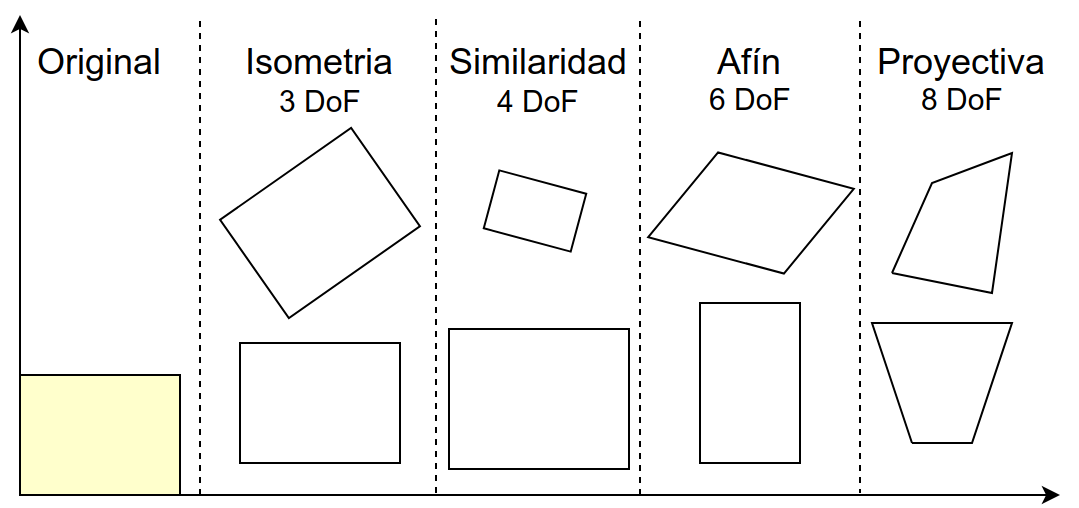
\includegraphics[width=14.5cm]{transformaciones}
	\caption[Tipos de transformaciones geométricas]{Tipos de transformaciones geométricas}
	\label{imagen:transformaciones}
\end{figure}

Las transformaciones proyectivas, al igual que las anteriores puede ser descompuesta en una serie de transformaciones de menor jerarquía, tal y como se muestra en la ecuación X para la proyectiva.

\begin{displaymath}
\mathrm{H} = \mathrm{H}_\mathsf{S} \mathrm{H}_\mathsf{A} \mathrm{H}_\mathsf{P} = 
\begin{bmatrix}
{s\vec{R}}&{\vec{t}}\\
{\vec{0}}&{1}
\end{bmatrix}
\begin{bmatrix}
{\vec{K}}&{\vec{0}}\\
{\vec{0}}&{1}
\end{bmatrix}
\begin{bmatrix}
{\vec{I}}&{\vec{0}}\\
{\vec{v}}&{u}
\end{bmatrix} =
\begin{bmatrix}
{\vec{A}}&{\vec{t}}\\
{\vec{v}}&{u}
\end{bmatrix}
\end{displaymath}

Donde los sub-índices de las matrices corresponden con S = similaridad, A = Afín, P = Proyectiva. $\vec{R}$ es una matriz de rotación (no singular) $2\times2$,  $\vec{K}$ es una matriz $2\times2$ triangular superior normalizada tal que det$\vec{K}=1$ (para remover la escala y rotación), $\vec{t}$ es un vector de translación de 2 componentes, $\vec{I}$ es una matrix identidad $2\times2$, $\vec{v}$ es un vector de 2 componentes, $\vec{A}$ es una matriz no singular y $u\neq0$.

Las transformaciones proyectivas también cumplen con las siguientes aserciones: El inverso de una homografía, es también una homografía. La composición de dos homografía es una homografía. En base a esto, siempre es posible encontrar una matriz de transformación que pueda relacionar dos planos

\begin{figure}[H]
	\centering
	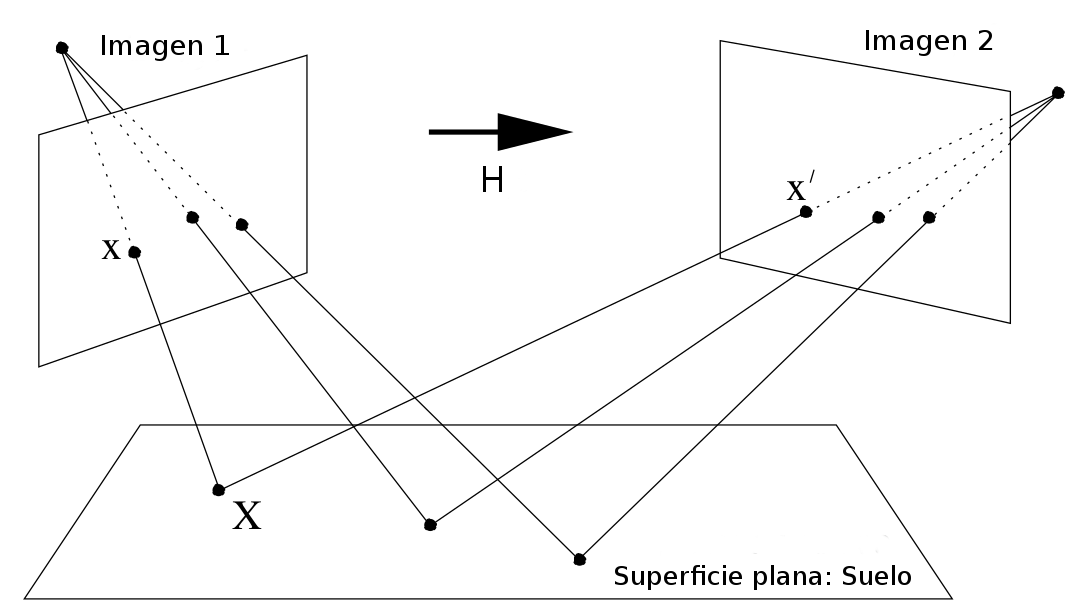
\includegraphics[width=12cm]{planos}
	\caption[Ejemplo de transformación geométrica]{Ejemplo de transformación geométrica}
	\label{imagen:planos}
\end{figure}

%%%%%%%%%%%%%%%%%%%%%%%%%%%%%%%%%%%%%%%%%%%%%%%%%%%%%%%%%%
\subsection{Estimación de Homografía}
\begin{displaymath}
x' = \frac{x'_1}{x'_3} = \frac{h_{11}x+h_{12}y+h_{13}}{h_{31}x+h_{32}y+h_{33}}, \qquad y' = \frac{x'_2}{x'_3} = \frac{h_{21}x+h_{22}y+h_{23}}{h_{31}x+h_{32}y+h_{33}}
\end{displaymath}
\begin{displaymath}
{x' ( h_{31}x+h_{32}y+h_{33} ) = h_{11}x+h_{12}y+h_{13}}
\end{displaymath}
\begin{displaymath}
{y' ( h_{31}x+h_{32}y+h_{33} ) = h_{21}x+h_{22}y+h_{23}}
\end{displaymath}

%%%%%%%%%%%%%%%%%%%%%%%%%%%%%%%%%%%%%%%%%%%%%%%%%%%%%%%%%%
\section{Generación de sub-mosaicos}

\begin{algorithm}[H] %or another one check
	\caption{Registro de imágenes}
	\SetAlgoLined
	$I_{i+1}$ $\equiv$ Imagen nueva\;
	$I_{i}$ $\equiv$ ultima imagen añadida al mosaico\;
	$V_{i}$ $\equiv$ vecinos de $I_{i}$\;
	\While{puntos emparejados $\ge$ 4}{
		Emparejar puntos de $I_{i+1}$ con $I_{i}$\;
		\If{$I_{i}$ tiene vecinos}{
			\ForEach {vecino de $I_{i}$}{
				Emparejar puntos de $I_{i+1}$ con $V_{i}$\;
			}
		}
		descartar malos emparejamientos\;
		aplicar busqueda sectorizada\;
		\If{puntos totales emparejados $\le$ 3}{
			modificar criterio para descartar\;
			\If{criterio para descartar llega al minimo}{
				terminar \tcp*{no es posible emparejar imagen}
			}
		}
	}
\end{algorithm}


\subsection{Selección de imagen de referencia}
Prueba

\subsection{Matriz de transformación promedio}

\begin{algorithm}[H] %or another one check
	\caption{Calculo de matriz de homografia promedio}
	\SetAlgoLined
	
	\While{no se alcanza el maximo de iteraciones}{
		seleccionar 4 puntos aleatorios del primer sub-mosaico\;
		seleccionar los 4 puntos correspondientes en el segundo sub-mosaico\;
		calcular el punto medio para cada par de puntos correspondientes\;
		calcular la transformacion desde los puntos del primer sub-mosaico hasta los puntos medios\;
		aplicar transformacion en el primer sub-mosaico\;
		calcular error de distorsión en el primer sub-mosaico\;
		\eIf{el error es menor que el mas bajo obtenido}{
			guardar el error como el mas bajo\;
			guardar la matriz de transformación como la mejor\;
		}{
		restaurar valores del primer sub-mosaico\;
	}
}
\end{algorithm}


\section{Corrección euclidiana}
Prueba

\section{Resultados}
Resumen

\section{Resumen}
Resumen



